\section{\texorpdfstring{$\chi_{b1}$}{chib1} and \texorpdfstring{$\chi_{b2}$}{chib2} yields ratio}
\label{sec:ratio}

\begin{figure}[H]
  \setlength{\unitlength}{1mm}
  \centering
  \begin{picture}(75,60)
    %
     \put(0,0){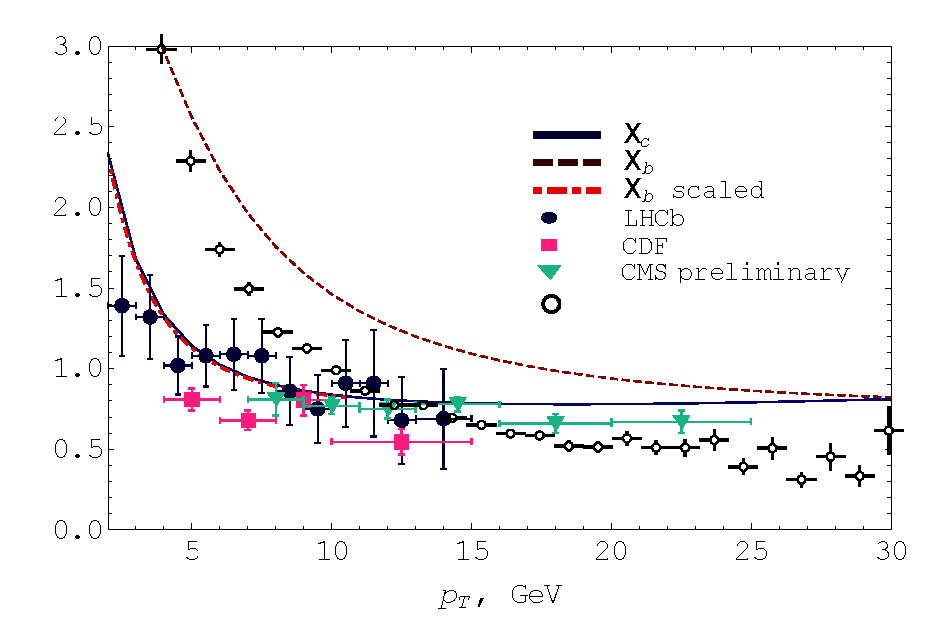
\includegraphics[width=75mm, height=60mm]{ratio/theory}}


     \put(-1,22){\begin{sideways}$\sigma({\chi_2})/\sigma({\chi_1}$)\end{sideways}}
     \put(46,30){\tiny $\chi_b$ scaled}
     \put(45,27){\tiny (this study, MC data)}

    % \graphpaper[5](0,0)(75, 60)
  \end{picture}
  \caption {\small This figure is taken from~\cite{Likhoded:2012hw} and shows
  transverse momentum distributions of the
$d\sigma\left[\chi_{2}\right]/d\sigma[\chi_{1}]$ ratio. Solid and dashed lines
stand for charmonium and bottomonium mesons. The dot-dashed line corresponds to
the rescaled bottomonium ratio:
$\sigma_{b2}/\sigma_{b1}(M_{\chi_c}/M_{\chi)b}\,p_T)$. The experimental results
for charmonium from LHCb \cite{LHCb-PAPER-2013-028} are shown with dots,
CDF~\cite{CDF:2007bra} --- with rectangles, and CMS~
\cite{CMS-PAS-BPH-11-010} --- with triangles. The scaled transverse momentum
distribution of \chib on Monte-Carlo data from this study is shown with open
circles. As it is seen, it almost matches the bottomonium curve. Thus the
results of this work have a reason to be used for fixing the fractions of
\chibone and \chibtwo yields on data. }
  \label{fig:frac:ratio}
\end{figure}

The \chibone and \chibtwo ratio is measured by the following formula in
specified transverse momentum intervals of \Y1S:
\begin{equation}
    \frac{N_{\chibtwo}^{data}}{N_{\chibone}^{data}} = \frac{\sigma(\chibtwo)}{\sigma(\chibone)}
    \frac{Br(\chibtwo\to\Upsilon\gamma)}{Br(\chibone\to\Upsilon\gamma)}\frac{\eps_{\chibtwo}}{\eps_{\chibone}}
\label{eqn:mc_ratio}
\end{equation}
, where $\sigma(\chibtwo) / \sigma(\chibone)$ is a ratio
from~\cite{Likhoded:2012hw}.

\begin{table}[H]
\caption{Branching ratios}
\centering
\begin{tabular}{l}
$Br_1[1P, 1S] = 35\% \pm 8\%$ \\
$Br_2[1P, 1S] = 22\% \pm 4\%$ \\
$Br_1[2P, 1S] = 8.5\% \pm 1.3\%$ \\
$Br_2[2P, 1S] = 7.1\% \pm 1\%$ \\
$Br_1[2P, 2S] = 21\% \pm 4\%$ \\
$Br_2[2P, 2S] = 16\% \pm 2.4\%$ \\
\end{tabular}
\label{tab:branching}
\end{table}


\begin{table}[H]
\caption{Summary of \chibone yield fraction ($\lambda_{\chi_{b1}(1,2P)}$)
determination  in data fits.}
\scalebox{0.6}{
	\begin{tabular}{lcccccccc}
	& \multicolumn8{c}{\OneS transverse momentum interval, \gevc} \\
	 & 6 --- 8 & 8 --- 10 & 10 --- 12 & 12 --- 14 & 14 --- 18 & 18 --- 22 & 22 --- 30 & 18 --- 30 \\
	\hline
	$\frac{\sigma{\chibtwo}}{\sigma{\chibone}}$  & 1.77 $\pm$ 0.17 & 1.50 $\pm$ 0.10 & 1.30 $\pm$ 0.10 & 1.15 $\pm$ 0.05 & 1.05 $\pm$ 0.05 & 0.95 $\pm$ 0.05 & 0.85 $\pm$ 0.05 & 0.90 $\pm$ 0.10 \\

	$\frac{\eps_{\chibtwo(1P)}}{\eps_{\chibone(1P)}}$  & 0.991 $\pm$ 0.013 & 1.029 $\pm$ 0.017 & 0.931 $\pm$ 0.019 & 0.970 $\pm$ 0.025 & 0.963 $\pm$ 0.028 & 1.03 $\pm$ 0.04 & 0.96 $\pm$ 0.05 & 1.003 $\pm$ 0.034 \\
	$\frac{\eps_{\chibtwo(2P)}}{\eps_{\chibone(2P)}}$  & 0.885 $\pm$ 0.015 & 0.873 $\pm$ 0.017 & 0.952 $\pm$ 0.021 & 0.978 $\pm$ 0.026 & 0.961 $\pm$ 0.032 & 1.00 $\pm$ 0.06 & 0.83 $\pm$ 0.07 & 0.95 $\pm$ 0.05 \\


	\rule{0pt}{4ex}$\frac{N_{\chibtwo(1P) \rightarrow \Y1S \gamma}}{N_{\chibone(1P) \rightarrow \Y1S \gamma}}$  & 1.11 $\pm$ 0.34 & 0.97 $\pm$ 0.29 & 0.76 $\pm$ 0.23 & 0.70 $\pm$ 0.21 & 0.64 $\pm$ 0.19 & 0.61 $\pm$ 0.18 & 0.51 $\pm$ 0.16 & 0.57 $\pm$ 0.18 \\

	$\frac{N_{\chibtwo(2P) \rightarrow \Y1S \gamma}}{N_{\chibone(2P) \rightarrow \Y1S \gamma}}$  & 1.31 $\pm$ 0.30 & 1.09 $\pm$ 0.24 & 1.03 $\pm$ 0.23 & 0.94 $\pm$ 0.20 & 0.84 $\pm$ 0.18 & 0.80 $\pm$ 0.18 & 0.59 $\pm$ 0.14 & 0.71 $\pm$ 0.17 \\

	\rule{0pt}{4ex}$\alpha_{\chiboneOneP}$  & 0.47 $\pm$ 0.08 & 0.51 $\pm$ 0.07 & 0.57 $\pm$ 0.07 & 0.59 $\pm$ 0.07 & 0.61 $\pm$ 0.07 & 0.62 $\pm$ 0.07 & 0.66 $\pm$ 0.07 & 0.64 $\pm$ 0.07 \\
	$\alpha_{\chiboneTwoP}$  & 0.43 $\pm$ 0.06 & 0.48 $\pm$ 0.05 & 0.49 $\pm$ 0.06 & 0.52 $\pm$ 0.05 & 0.54 $\pm$ 0.05 & 0.56 $\pm$ 0.06 & 0.63 $\pm$ 0.05 & 0.58 $\pm$ 0.06 \\
	\end{tabular}
}
\label{tab:ratio:lambda}
\end{table}

